\documentclass[12pt,aspectratio=2013]{beamer}
\setbeamertemplate{navigation symbols}{}
\setbeamertemplate{footline}[page number]
\title{ROCK implementation in Python\\
with Code by Victor Rielly}
\author{Adam Handwerger}
\date{}
\usetheme{default}
\usepackage{amsmath,amsfonts,amssymb}
\usepackage{natbib}
\usepackage{booktabs}
\usepackage{stmaryrd}
\usepackage{nopageno}
\usepackage{hyperref}
\usepackage{bookmark}
\usepackage{mathtools}
\usepackage{pdfpages}
\usepackage{geometry}
\usepackage{relsize}
\usepackage{graphicx}
\usepackage{xfrac}
\usepackage{dsfont}
\usepackage{tikz}
\usepackage{tikz} \usetikzlibrary{angles,quotes}
\usepackage{relsize}
\usepackage{caption}
%\usepackage[style=apa]{biblatex}
\usepackage[utf8]{inputenc}
\begin{document}
\frame{\titlepage}
\begin{frame}{Recount ROCK Objective}
    We seek an f which minimizes $J(f)=$\\
    \begin{equation}
    \biggl\{\sup\limits_{v(t):\parallel v(t) \parallel=1} \left[\left(\int\limits_a^b \left(\dot{x}(t)-f(x(t))\right)^{\top}v(t) dt \right)^2\right]+\lambda\! \parallel \!f\!\parallel^2\biggr\}
    \end{equation}
    \vspace{.25cm}
where $f \in$ an vvRKHS $\text{ and } v(t)$ is d-dimensional test function from\\
a finite dimensional vvRKHS, V with a p-dimensional feature map, $\phi_{\tau}$.\\ 
\end{frame}
\begin{frame}{Using ROCK to reframe problem}
Using the the theory of ROCK, (1) can be reframed as solving the\\
following linear system for $\alpha$:\\
\vspace{.5cm}
\begin{equation}
\left(M+\lambda I\right)\alpha=y, \text{ where } y\in{\mathbb{R}^{npd}}
\end{equation}
\\
\vspace{.25cm}
Thus we will need to construct the matrix M and the vector y,\\
but first we will define the block diagonal matrix $\Psi(t)$.\\
\end{frame}
\begin{frame}{The Test Function Matrix $\Psi(t)$}
If p is the dimension of the feature map $\phi_\tau$ for V, and $m_i$ is the\\
number of samples of each trajectory then for each trajectory, there\\
is a corresponding block in $\Psi$ given by\\
$$
\psi_{i,i}=[\psi_i(t^i_1),\dots,\psi_i(t^i_{m_{i}})] \in\mathbb{R}^{pxm_i}
$$
\end{frame}
\begin{frame}{Code for Constructing $\psi_i$ using Legendre Polynomials\\ as Components of the Test Functions}
For this example the vector-valued test function $v(t)$ for trajectory i\\ 
has components which are given by the scaled/shifted Legendre\\
Polynomials defined on time interval $[a_i,b_i]$. Each component is found \\
recursively up to order p using a the well known recursion formula\\
for Legendre Polynomials. The following code calculates $\psi_{i}(t^i)$\\
$\text{and its time derivative, } \dot{\psi}_{i}(t^i)$ for each element in the time array\\
with $t^i \in [a_i,b_i]$. Note that $P_1(t)\propto t$ so that the recursion can start\\
on each element of the time array.
\end{frame}
\begin{frame}
    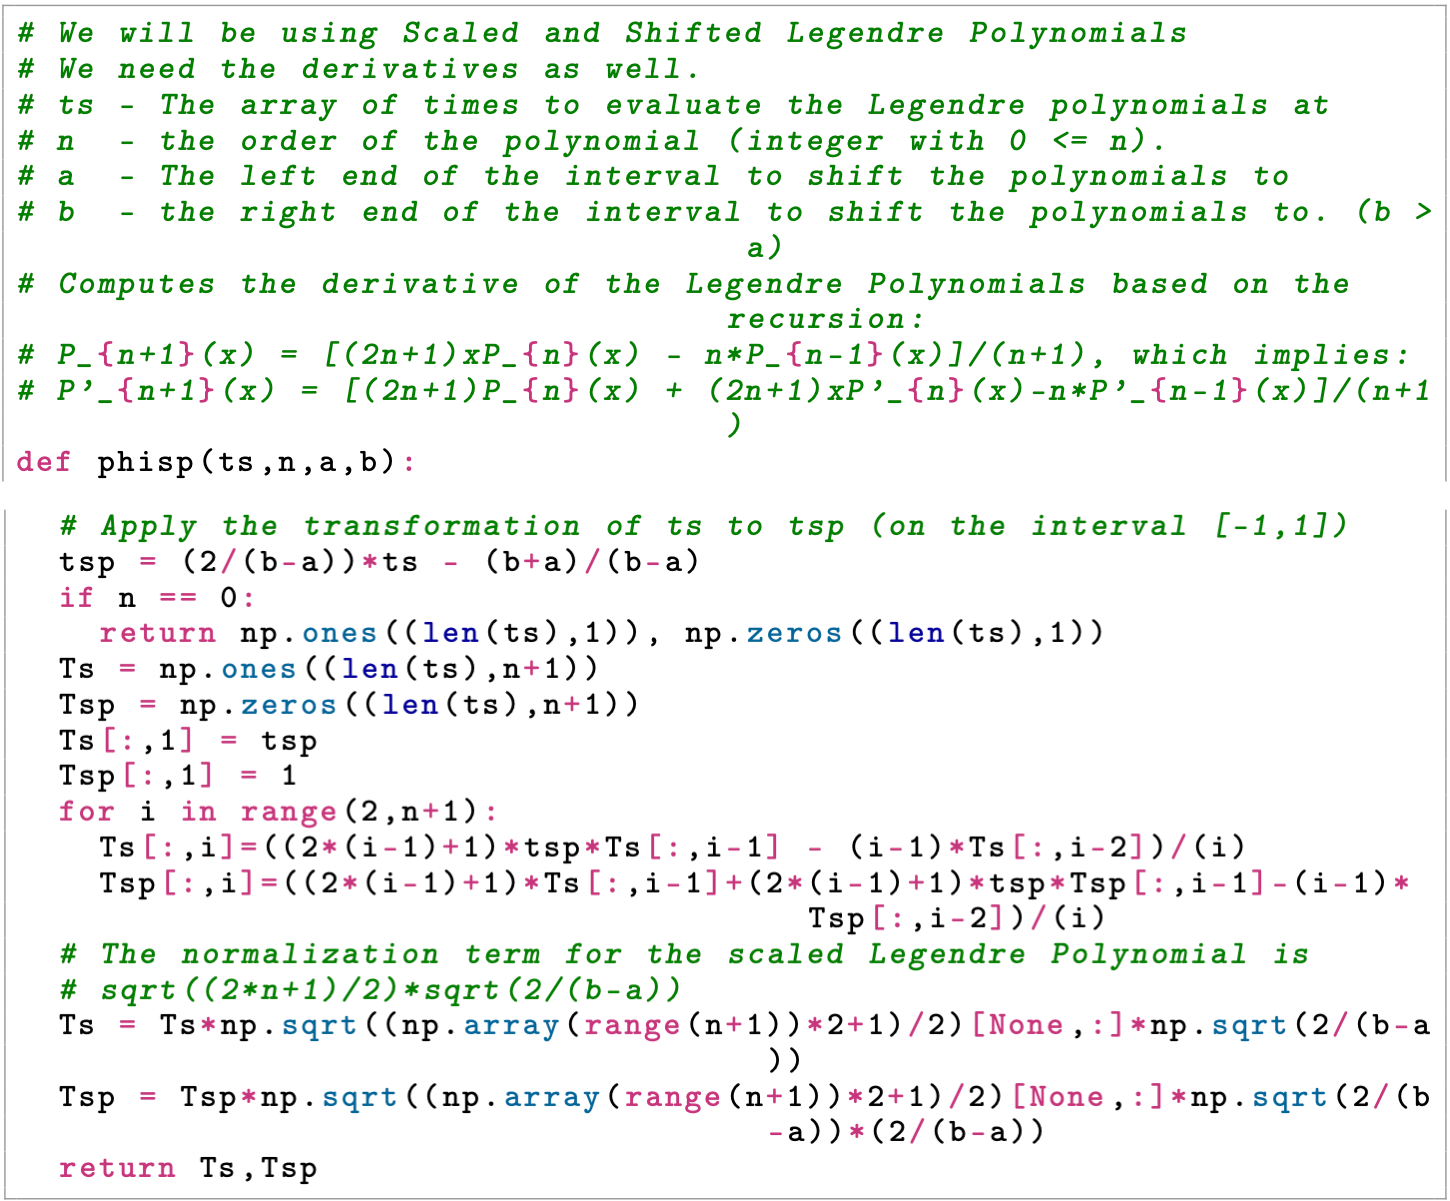
\includegraphics[scale=.2]{scribe_image(1).png}
\end{frame}
\begin{frame}{The Vector $y \in \mathbb{R}^{npd}$}
To contruct the vector y we stack the n vectors $y_i$ given by\\
$$
y_i=\int\limits^{b^i}_{a^i} \Psi_i(t)\dot{x}^i(t) dt
$$
which themselves are stacked vectors. For each i there are p vectors\\
$y_{ij}$ which are given by\\
$$
y_{ij}=x_i(b_i)[\psi(b_i)]_j-x_i(a_i)[\psi(a_i)]-\int\limits^{b^i}_{a^i} x_i(t)\left[\dot{\psi}_i(t)\right]_j dt \in \mathbb{R}^d
$$
where $j \in \{1,2,...,p\}$
\end{frame}
\begin{frame}{Construction of y Using Matrix Multiplication}
We first construct two related matrices $QPhi \text{ and } QphiD$.\\
Both matrices are block diagonal and are contained in $\mathbb{R}^{pn\times (\sum_i^n m_i)}$,\\
with each block given by\\
\vspace{.25cm}
$\hspace{3cm}QPhi_{i,i}=[q^i_1 \Psi_i(t_1^i),..., q^i_{m_{i}} \Psi_i(t^i_{m_{i}})]$\\
\vspace{.25cm}
and likewise,\\
\vspace{.25cm}
$QPhiD_{i,i}=[-\Psi_i(t_1^i)-q^i_1 \dot{\Psi}_i(t_1^i), -q^i_2 \dot{\Psi}_i(t_2^i),...,-\Psi_i(t_{m_{i}}^i)-q^i_1 \dot{\Psi}_i(t_{m_{i}}^i)]$\\
\vspace{.25cm}
The $q^i$ are the quadrature weights which are determined by\\
integration method. Notice that the first and last terms in $QPhiD_{i,i}$\\
have an additive boundary term which is addressed in the Python code.\\
\end{frame}
\begin{frame}{Construction of y Continued}
Let $X=(x_1,...,x_n)$ be the set of data from the n trajectories. Define\\
Y as the y vector, as defined before expect now partially unstacked as\\
a matrix with with d columns.\\
\vspace{.35cm}
Then,
\begin{equation}
Y=X \cdot  QPhiD^{\top}
\end{equation}
where $\cdot$ implies matrix-matrix multiplication. The following code\\
constructs $QPhi$ and $QPhiD$ and then determines Y in Python.
\end{frame}
\begin{frame}
    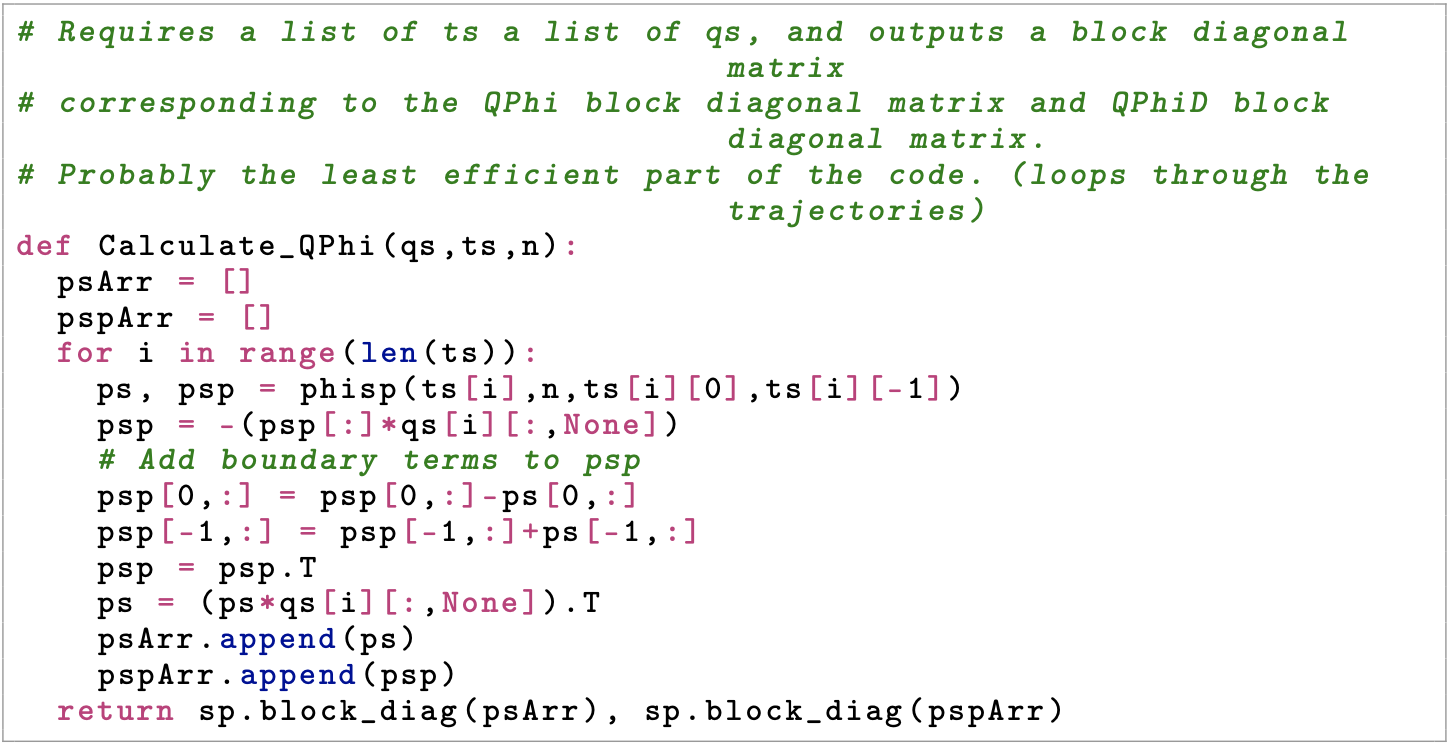
\includegraphics[scale=.2]{scribe_image(2).png}
    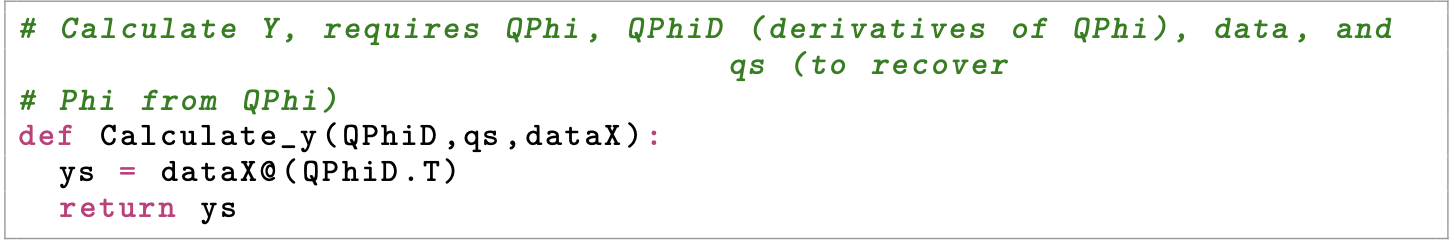
\includegraphics[scale=.2]{scribe_image(3).png}
\end{frame}
\begin{frame}{The Matrix $M \in \mathbb{R}^{pnd\times pnd}$}
M is block diagonal matrix with blocks given by
\begin{equation}
M_{ij}=\iint K(x_i(s),x_j(t)) dsdt
\end{equation}
In (4) above K is a matrix-valued kernel. In the case that\\
$K=k(x_i,x_j)\cdot I_d$ (4) becomes\\
\begin{equation}
M_{ij}=\iint k(x_i(s),x_j(t)) dsdt\otimes I_d
\end{equation}
The double integral in M can be evaluated numerically in Python using
a quadrature approximation method.
\end{frame}
\begin{frame}{The Vectorized Guassian Kernel}
A kernel function can be constructed in Python which inputs\\
matrices $X,Y \in \mathbb{R}^{d\times \sum_i^n m_i}$ of vectors and outputs the scaler\\
kernel value for each element of the output matrix. The\\
following Python code accomplishes this task:\\
\vspace{.2cm}
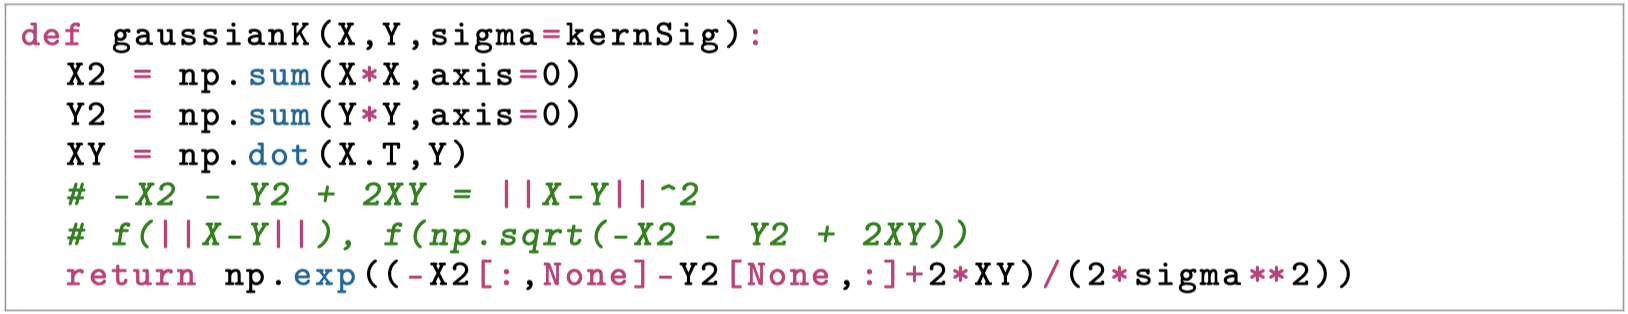
\includegraphics[scale=.2]{scribe_image(4)}\\
\vspace{.2cm}
This technique of reshaping the vector 'X2','Y2' with 'None' in the\\
index allows numpy to calculate the Gram matrix without explicitly\\
using 'for' loops. This vectorization of the code leads to increased\\
efficiency.\\
\end{frame}
\begin{frame}{Construction of the M Matrix using Matrix Multiplication}
In order to contruct M we will need the Gram Matrix, G from the dataset X.
The matrix $G \in \mathbb{R}^{(\sum_i^n mi_i\times\sum_i^n mi_i)}$ is defined as \footnote{we take dataX=dataY}\\
$$
G=\begin{pmatrix}
k(x_{1,1},x_{1,1}) & k(x_{1,1},x_{1,2}) &\cdots &k(x_{1,1},x_{n,m_n})\\
\vdots       &           \vdots&       &\vdots\\
k(x_{n,m_n},x_{1,1})&k(x_{n,m_n},x_{1,2})&\cdots&k(x_{n,m_n},x_{n,m_n})\\
\end{pmatrix}
$$
\vspace{-.3cm}
Then M is given by the matrix product\\
\vspace{.05cm}
\begin{equation}
M=QPhi\cdot(G\cdot QPhi^{\top})
\end{equation}
\vspace{.05cm}
The following Python code implements this multiplication with\\
the Guassian kernel.\\
\end{frame}
\begin{frame}{Python Code for Constructing M}
    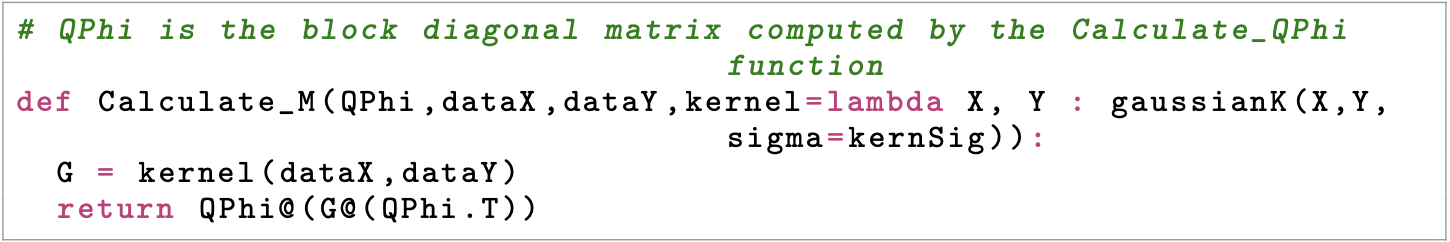
\includegraphics[scale=.2]{scribe_image(5).png}
\end{frame}
\begin{frame}{Solving for $\alpha$}

We now solve for the partial-unstacked $\alpha \in \mathbb{R}^{np\times d}$\\
with the substitution, $Y^{\top}$ for y in equation (1).\\
\vspace{.25cm}
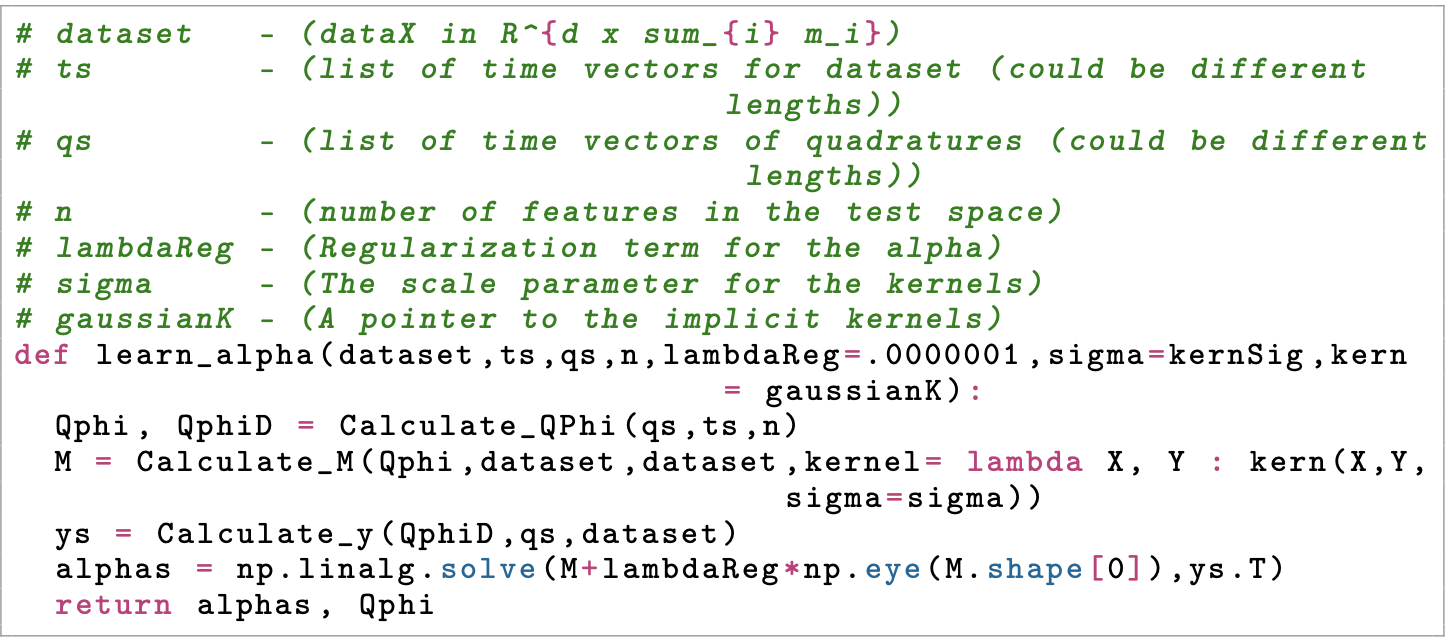
\includegraphics[scale=.2]{scribe_image(6).png}
\end{frame}
\begin{frame}{Calculation of f at New Data Points}
Evaluating f along a trajectory outside the training set requires
only matrix multiplications:
\begin{equation}
f=\alpha^{\top}\cdot((G\cdot(QPhi^{\top}))^{\top})
\end{equation}
where G and QPhi are contructed once again with the new data\\
points. The Python code for this calculation is below:\\
\vspace{.35cm}
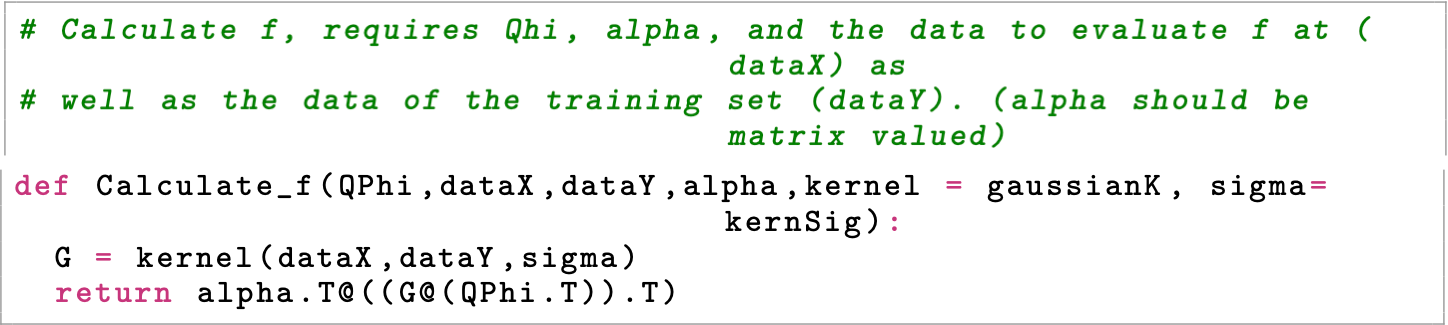
\includegraphics[scale=.2]{scribe_image(7).png}
\end{frame}
\end{document}